\chapter{Návrh a implementácia aplikácie}

Aby aplikácia podporovala čo najväčšie množstvo zariadení, bude minimálna podporovaná verzia Androidu 4.4, a kedže sa jedná a natívne vyvíjanú aplikáciu, použijeme oficiálny nástroj Android Studio.  Za programovací jazyk bola zvolená kombinácia Javy a Kotlinu, keďže sú podporované zvoleným IDE od inštalácie a majú veľkú komunitu spolu s množstvom knižníc. Serverovú časť aplikácie má na starosti služba Heroku, na ktorej je nasadená Node.JS aplikácia, ktorá sa správa ako most medzi MongoDB databázou ktorú poskytuje služba mlab.com \ref{obr3.4}. Na rozdiel od Slacku a JIRA, táto aplikácie ponúkne minimalistické používateľské prostredie a jednoduchosť. V návrhu popíšeme klientskú aj serverovú časť architektúry aplikácie.


\vspace{10pt}
\begin{figure}[H]
    \begin{center}
        \begin{minipage}{0.9\linewidth}
            \begin{center}
                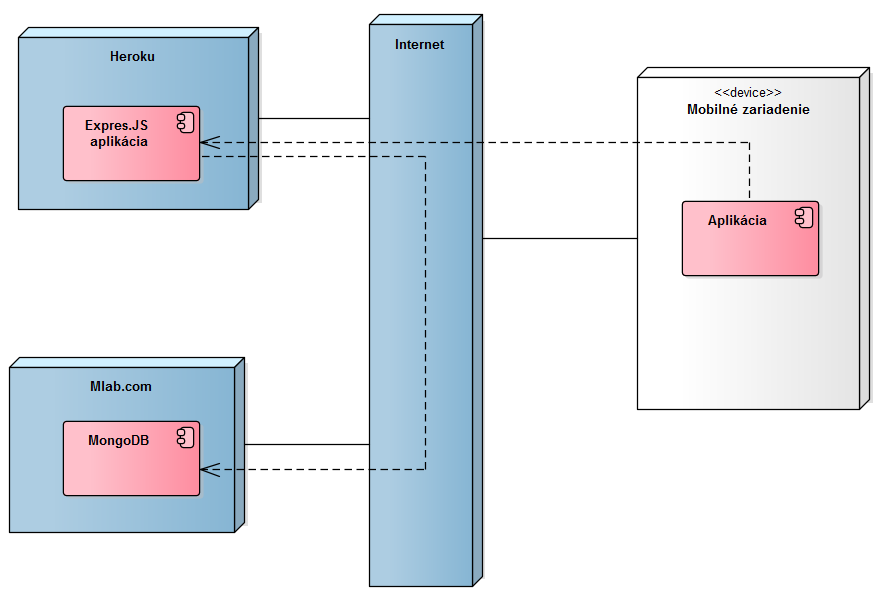
\includegraphics[width=0.9\textwidth]{images/deploy.png}
                \caption{Diagram nasadenia}
                \label{obr3.4}
            \end{center}
        \end{minipage}
    \end{center}
\end{figure}
\vspace{10pt}



\section{Architektúra aplikácie}
Pri návrhu aplikácie sme sa držali princípu oddelenia zodpovedností. Aby bol kód ľahšie rozšíriteľný a v budúcnosti znova použiteľný rozhodli sme sa pre našu aplikáciu aplikovať architektonický vzor
Model-View-Presenter. 
\vspace{10pt}
\begin{figure}[H]
    \begin{center}
        \begin{minipage}{0.9\linewidth}
            \begin{center}
                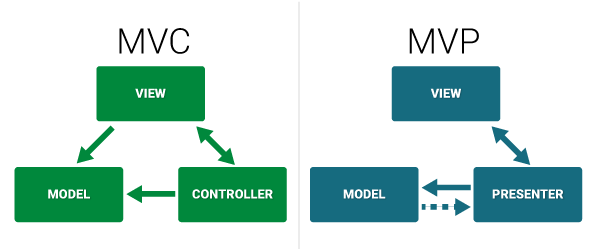
\includegraphics[width=0.9\textwidth]{images/MVC_MVP.png}
                \caption{Porovnanie MVP s MVC }
                \label{obr3.1}
            \end{center}
        \end{minipage}
    \end{center}
\end{figure}
\vspace{10pt}

Vzor nám umožní kompletne oddeliť biznis logiku od používateľského prostredia a to rozdelením ich zodpovedností \cite{mvpdef}.

\begin{description}
\item[Presenter]
 plní úlohu mostu medzi View a Modelom. Získava dáta z modelu a naformátované ich presúva do View modulu. Na rozdiel od MVC, rozhoduje aj o tom čo sa stane, keď nastane akcia vo view. 

\item[View]
 je implementovaný ako aktivita, ktorá si uchováva referenciu na presenter. Jediná vec ktorú view robí, je že volá metódy presentera.

\item[Model]
 v našej aplikácii predstavuje reprezentáciu dát, ktoré sú uložené v databáze, a aj s ňou komunikuje.

\end{description}

Aplikovanie vzoru (obr.\ref{obr3.1}) na Android je jednoduché. Vytvoríme rozhranie \textit{IView}   (obr.\ref{obr3.2}) ktoré reprezentuje všetky používateľské akcie, ako napríklad zobrazenie animácie, oznámenie o dokončení požiadavky na server a pod.

\vspace{10pt}
\begin{figure}[H]
    \begin{center}
        \begin{minipage}{0.9\linewidth}
            \begin{center}
                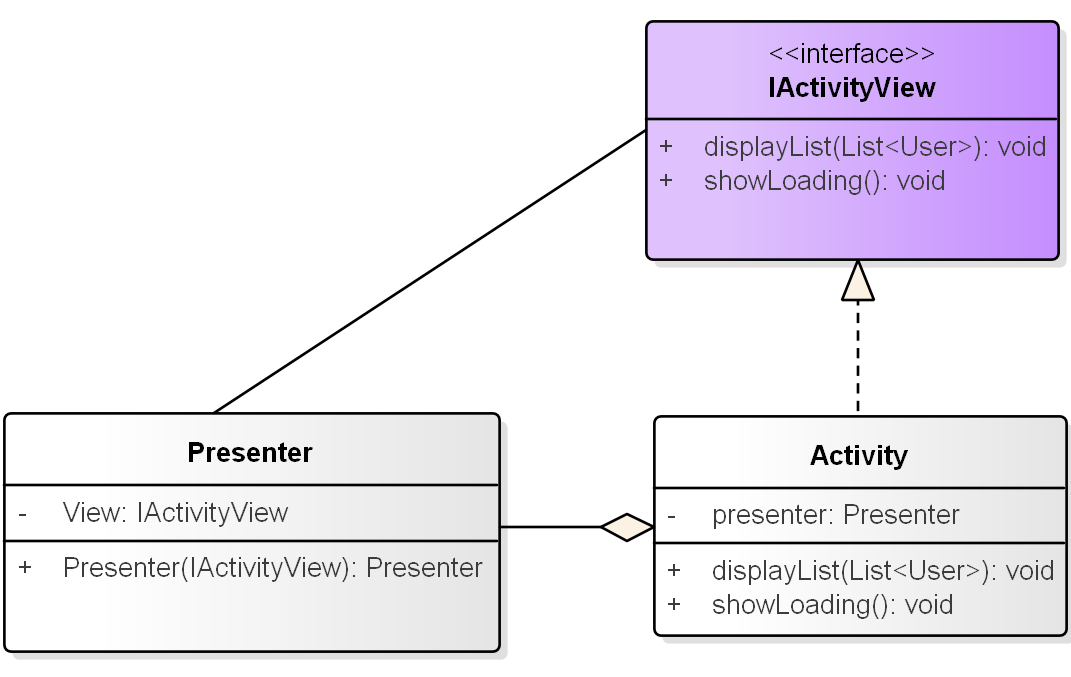
\includegraphics[width=0.9\textwidth]{images/mvpandroid.png}
                \caption{Nasadenie MVP v Androide }
                \label{obr3.2}
            \end{center}
        \end{minipage}
    \end{center}
\end{figure}
\vspace{10pt}

Presenter obsahuje objekt rozhrania, ktorý je aj parametrom konštruktora. Následne môže presenter volať metódy rozhrania. View implementuje rozhranie a všetky jeho metódy. V nich následne implementujeme kód, ktorý súvisí s View, ako je komunikácia s komponentami Androidu ako sú ListView, Progressbar a iné. Takýmto spôsobom oddelíme kód ktorý súvisí s Androidom od našej logiky, tým pádom presenter obsahuje kód, nezávislý na platforme na ktorý je možné napísať unit testy.

Aplikácia obsahuje triedu \textit{App}, ktorá je potomkom triedy \textit{Application}, ktorej inštancia je vytvorená skôr, ako ktorákoľvek iná trieda v balíčku aplikácie. To využívame na vytvorenie objektu klienta na komunikáciu s REST API, ktorý následne vkladáme do presentera aktivity, ktorá využíva sieťovú komunikáciu. Vytvorenie viacerých inštancií Http klienta by bolo zbytočné, keďže sa skladá z obsiahlych knižníc ako serializér a deserializér JSON objektov \textit{GSON}, Http knižnice \textit{OkHttp} a \textit{Retrofit}, ktorý uľahčuje prácu s REST API.

\section{Prihlasovacia obrazovka}

Prihlasovacia obrazovka slúži ako vstupná brána do aplikácie. Obsahuje polia pre email a heslo a tlačidlá prihlásenie, registráciu. Pri nesprávnom formáte emailu ktoré overuje regulárny výraz, alebo nevyplnených poliach, aplikácia používateľa upozorní zobrazením chybovej hlášky v príslušnom poli. Ak server vráti odpoveď o nesprávnom hesle,  používateľ je rovnako informovaný.

\vspace{10pt}


\begin{figure}[H]
    \begin{center}
        \begin{minipage}{0.7\linewidth}
            \begin{center}
     \frame{            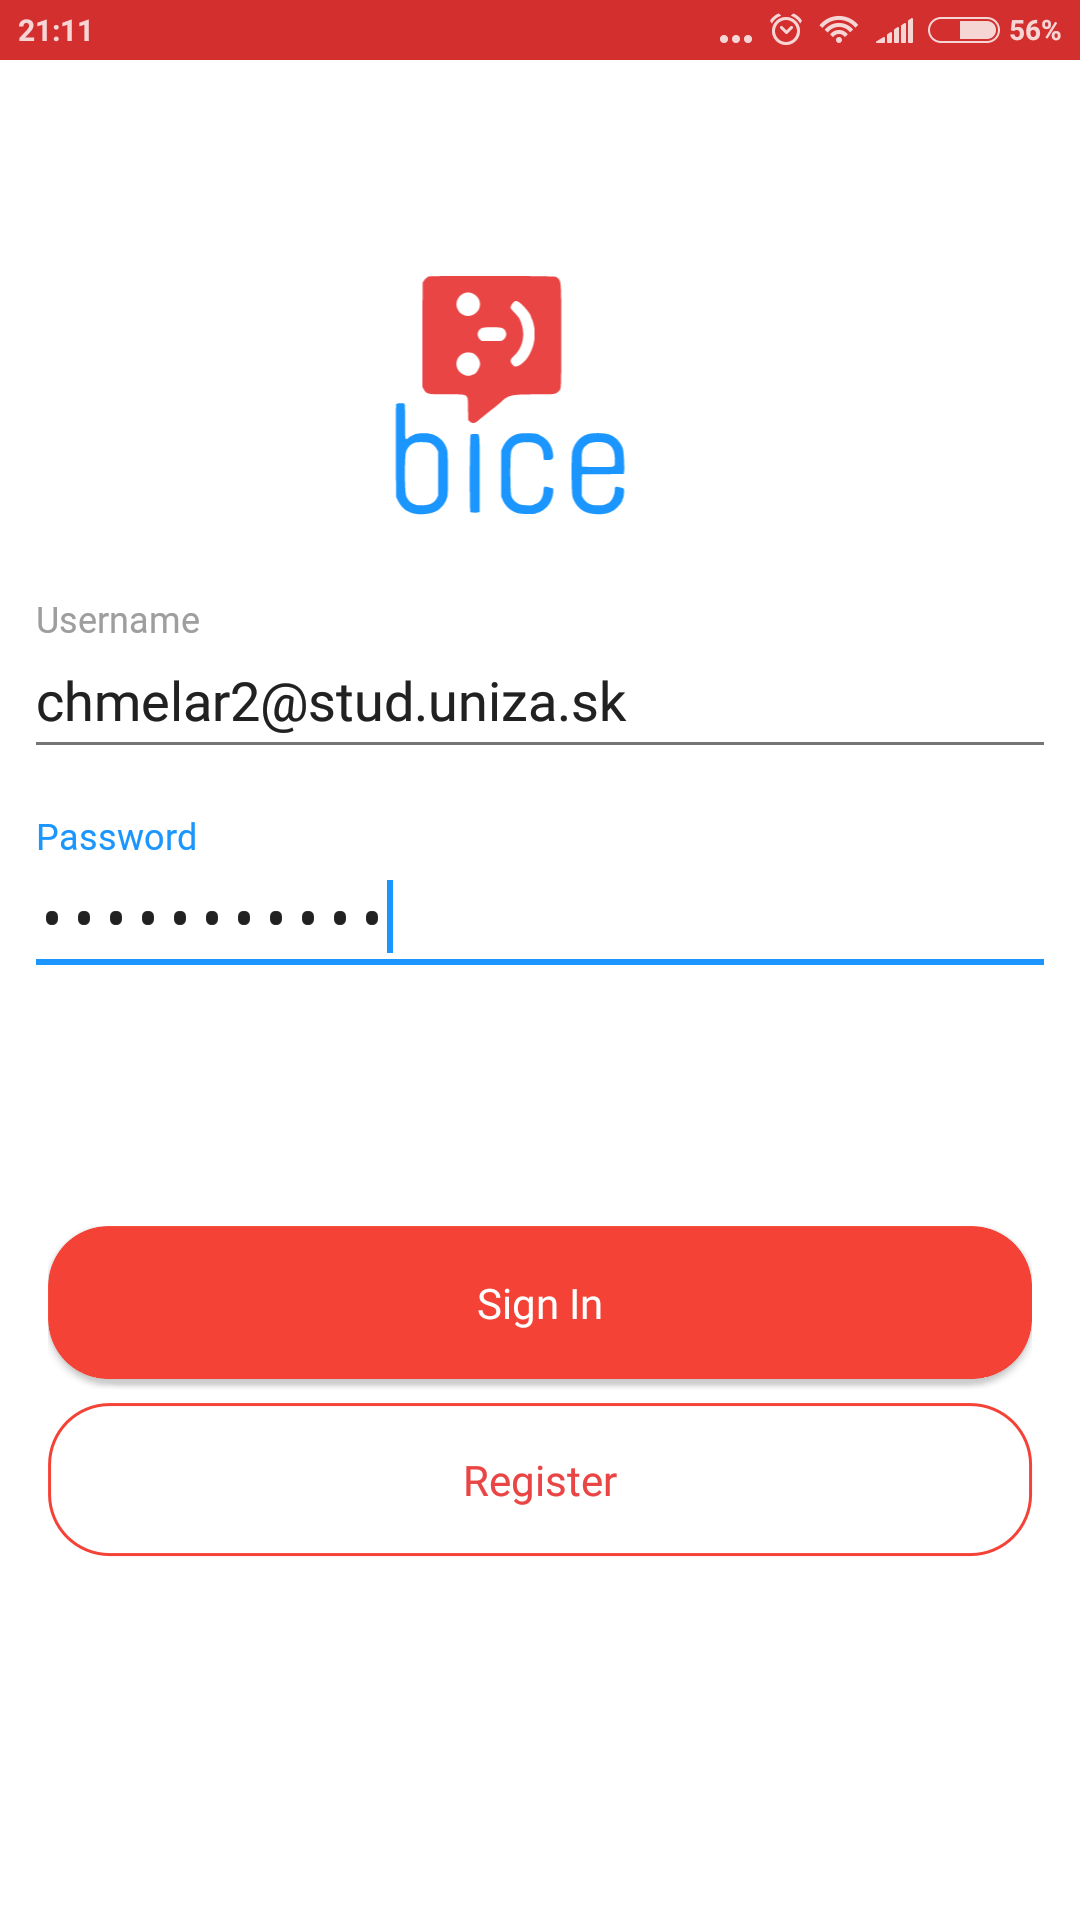
\includegraphics[width=0.7\textwidth]{images/login_screen.png} }
                \caption{Obrazovka prihlásenia}
                \label{obr3.3}
            \end{center}
        \end{minipage}
    \end{center}
\end{figure}




Pri inicializácii obrazovky vytvoríme inštanciu prezentéra, ktorý ako parametre akceptuje objekt typu \textit{IApiRoutes} na komunikáciu so serverom, a rozhranie \textit{IProjectsView}. Objekt \textit{IApiRoutes}  je vložený do prezentéra z hlavnej triedy \textit{App}. Trieda \textit{ProjectsActivity} implemetuje rozhranie \textit{IProjectsView} prezentéra, môže spracovať všetky správy odoslané prezentérom prostredníctvom rozhrania.

Po zadaní platnej adresy, ktorá je overovaná regulárnym výrazom, a heslom sa po stlačení červeného tlačítka na prihlásenie  zavolá metóda prezentéra, ktorá vola POST požiadavku, ktorej telo obsahuje JSON objekt s menom a heslom.

\vspace{10pt}
\begin{figure}[H]

    \begin{center}
        \begin{minipage}{1\linewidth}
            \begin{center}
               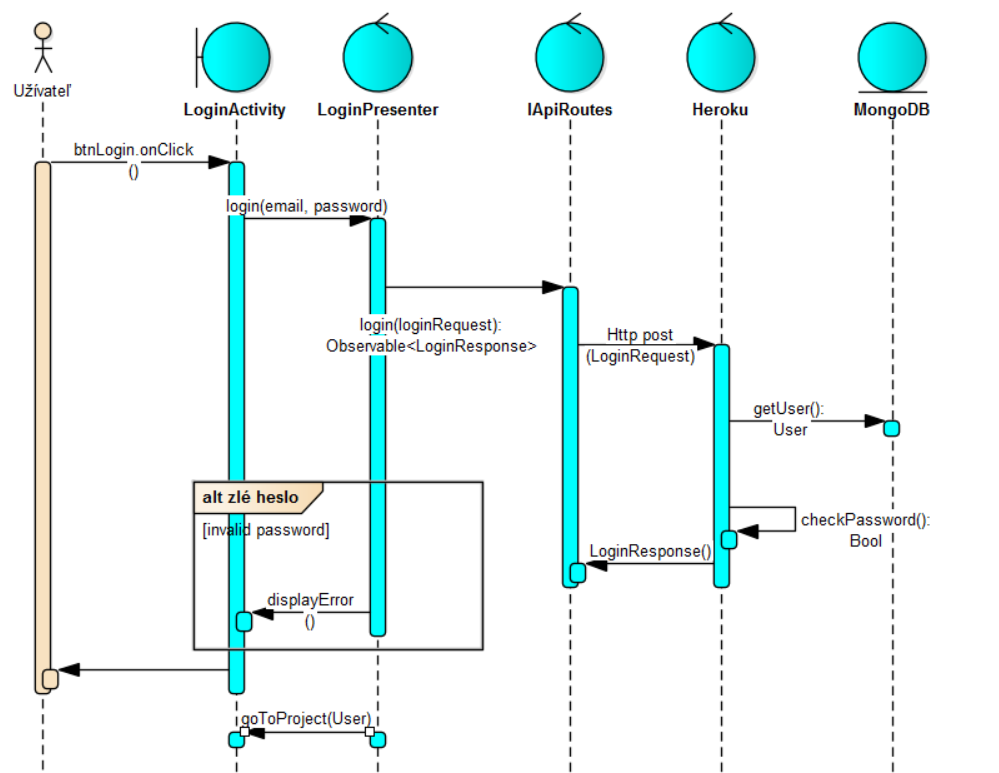
\includegraphics[width=1\textwidth]{images/login_rest.png}]   
                \caption{Sekvenčný diagram - Prihlasovanie }
                \label{obr3.5}
            \end{center}
        \end{minipage}
    \end{center}
    
\end{figure}
\vspace{10pt}

Server následne vyhľadá používateľa s požadovanou emailovou adresou. Spracuje heslo z tela požiadavky a porovná ho s kryptovanou verziou hesla. Po úspešnom porovnaní odošle server odpoveď v podobe JSON objektu s dátami o prihlásenom užívateľovi a \textit{JWT} kľúčom, ktorým sa môžeme identifikovať na serveri po dobu 24 hodín. Kľuč sa vkladá do Http klienta, ktorý ho automaticky vloží do hlavičky nasledujúcich požiadaviek.

\section{Obrazovka projektov}
Prihlasovacia obrazovka odoslala identifikačné číslo všetkých projektov, ktoré má používateľ zapísané. Prezentér odošle požiadavku na koncový bod servera \textit{/projects/:id}, kde \textit{:id} nahradí číslo projektu. Postupne sa projekty zobrazia na hlavnej obrazovke (obr.\ref{obr3.6}), odkiaľ používateľ pristupuje ku konkrétnym projektom.

\vspace{10pt}
\begin{figure}[H]

    \begin{center}
        \begin{minipage}{0.7\linewidth}
            \begin{center}
               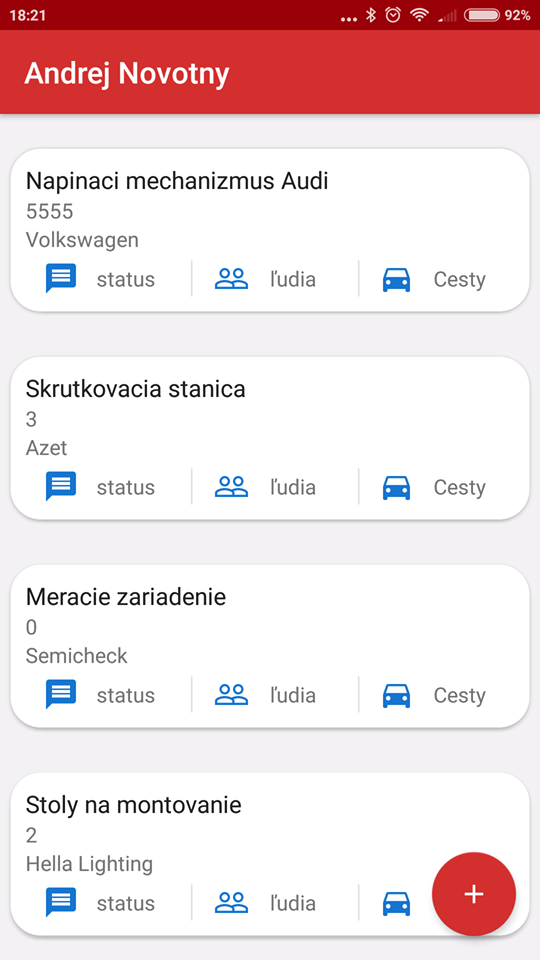
\includegraphics[width=0.7\textwidth]{images/screenz/main_screen.png}]   
                \caption{Obrazovka projektov}
                \label{obr3.6}
            \end{center}
        \end{minipage}
    \end{center}
    
\end{figure}
\vspace{10pt}


Po kliknutí na červené tlačítko so znakom ``+'' nás aplikácia presunie na obrazovku vytvorenia projektu (obr.\ref{obr3.7}).Obsahuje polia s nápovedou a automatickým dopĺňaním zamestnancov. Po vyplnení  požadovaných textových polí  odošle prezentér POST požiadavku na koncový bod  \textit{/projects/:id} s objektom JSON, ktorý obsahuje vyplnené dáta a čísla zamestnancov, ktorí budú pridaní do projektu. Následne sme presunutý na predošlú obrazovku. Aplikácia nás informuje o stave požiadavky \textit{toast} notifikáciou. 

\vspace{10pt}
\begin{figure}[H]

    \begin{center}
        \begin{minipage}{0.7\linewidth}
            \begin{center}
               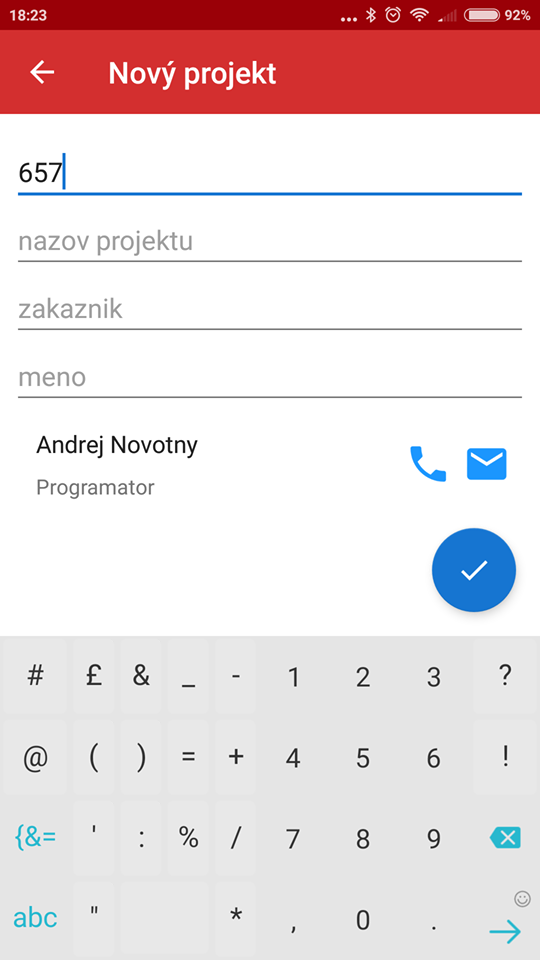
\includegraphics[width=0.7\textwidth]{images/screenz/projekt_new.png}]   
                \caption{Obrazovka vytvorenia projektu}
                \label{obr3.7}
            \end{center}
        \end{minipage}
    \end{center}
    
\end{figure}
\vspace{10pt}
 
\section{Detail projektov}

Detail obsahuje tri sekcie, medzi ktorými sa môžeme pohybovať kliknutím na prislúchajúcu záložku alebo potiahnutím prsta. Táto časť aplikácie je naprogramovaná v jazyku Kotlin. Obsahuje viacero komponentov ktoré sú veľmi podobné, ale s odlišnou logikou. Vďaka vlastnosti jazyka, ktorá umožňuje posielať funkciu ako parameter sme mohli znova použiť existujúce komponenty.

\subsection{Stav}

Zobrazuje posledné správy ktoré boli odoslané riešiteľmi projektu. Umožňuje odoslať aktualizáciu stavu prostredníctvom poľa v dolnej časti obrazovky. Podobne ako v predchádzajúcich obrazovkách, prezentér odosiela POST požiadavku na koncový bod  \textit{/projects/:id/comments} s textom komentára, číslom projektu a číslom užívateľa. Úspešné aktualizovaný stav sa zobrazí v zozname s časom odoslania a menom autora.

\vspace{10pt}
\begin{figure}[H]

    \begin{center}
        \begin{minipage}{0.7\linewidth}
            \begin{center}
               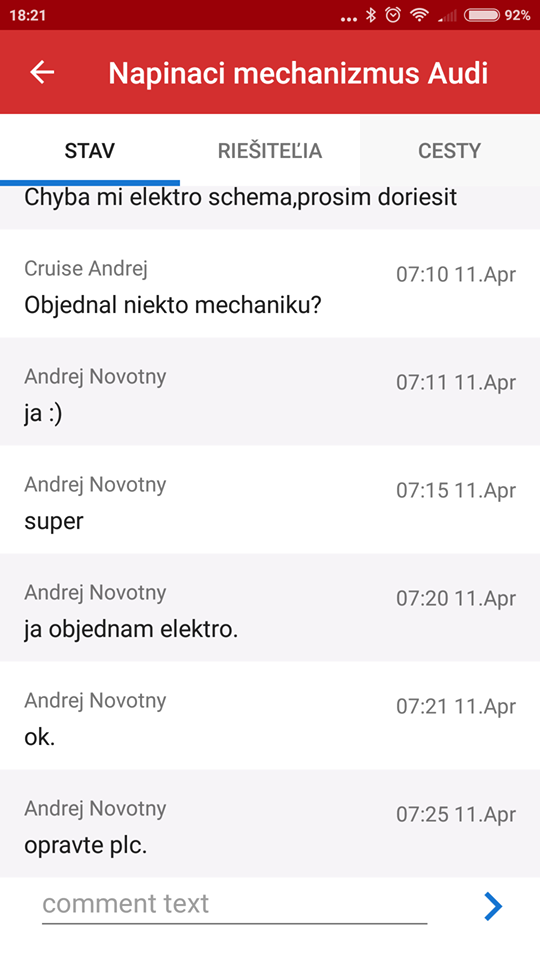
\includegraphics[width=0.7\textwidth]{images/screenz/stavy.png}]   
                \caption{Obrazovka stavov}
                \label{obr3.8}
            \end{center}
        \end{minipage}
    \end{center}
    
\end{figure}
\vspace{10pt}
\pagebreak
\subsection{Riešitelia}

V tejto záložke je vidieť všetkých používateľov, ktorí boli pridaní do projektu (obr.\ref{obr3.9}). Pri mene používateľa je zobrazená jeho pracovná pozícia, možnosť odoslať email alebo uskutočniť hovor. V spodnej časti obrazovky je možné pridať používateľa do projektu, alebo zorganizovať pracovné stretnutie. Kliknutím na ikonu pracovného stretnutia sa zobrazí dialóg na výber dátumu a času. Následne je používateľ presunutý na obrazovku s pred-vyplneným emailom na odoslanie (obr.\ref{obr3.10}). Email je adresovaný všetkým riešiteľom projektu.

\vspace{10pt}
\begin{figure}[H]

    \begin{center}
        \begin{minipage}{0.7\linewidth}
            \begin{center}
               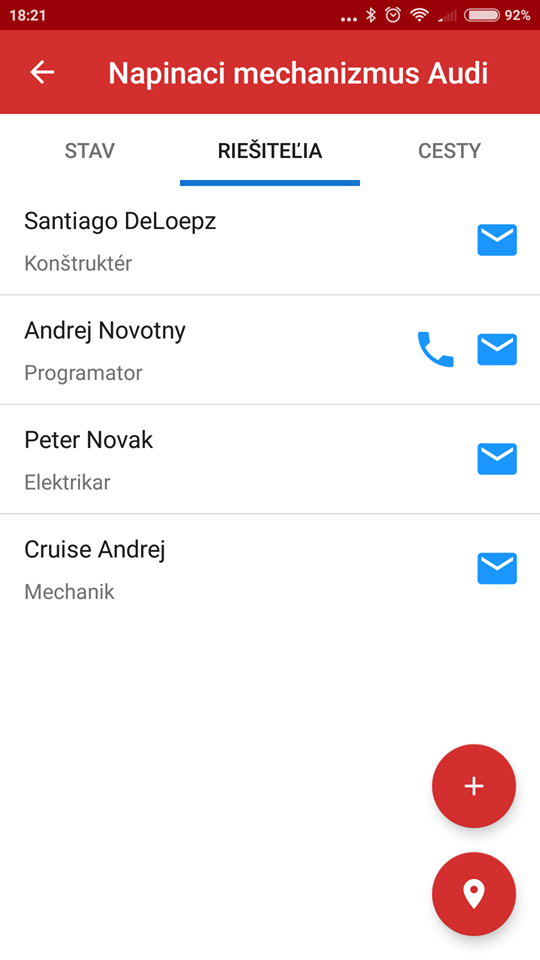
\includegraphics[width=0.7\textwidth]{images/screenz/riesitelia.png}]   
                \caption{Obrazovka riešiteľov}
                \label{obr3.9}
            \end{center}
        \end{minipage}
    \end{center}
    
\end{figure}
\vspace{10pt}

Výber emailového klienta je prenechaný na používateľa. Môže teda použiť akýkoľvek klient podľa vlastných preferencií

\vspace{10pt}
\begin{figure}[H]
  \centering
  \subfloat[Výber času stretnutia]{
    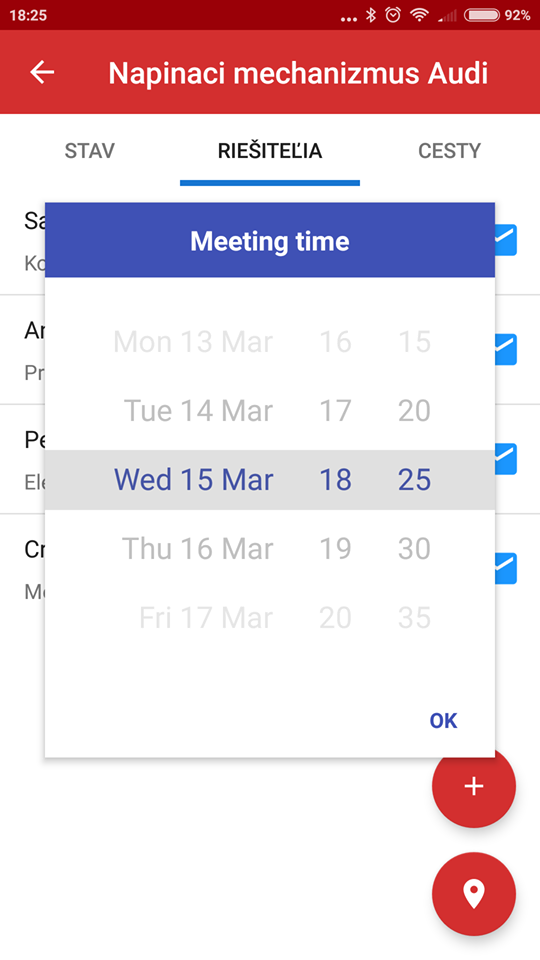
\includegraphics[width=0.4\textwidth]{images/screenz/meeting_datepicker.png}\label{obr3.11}
  }
  \hfill
  \subfloat[Pred-vyplnený email]{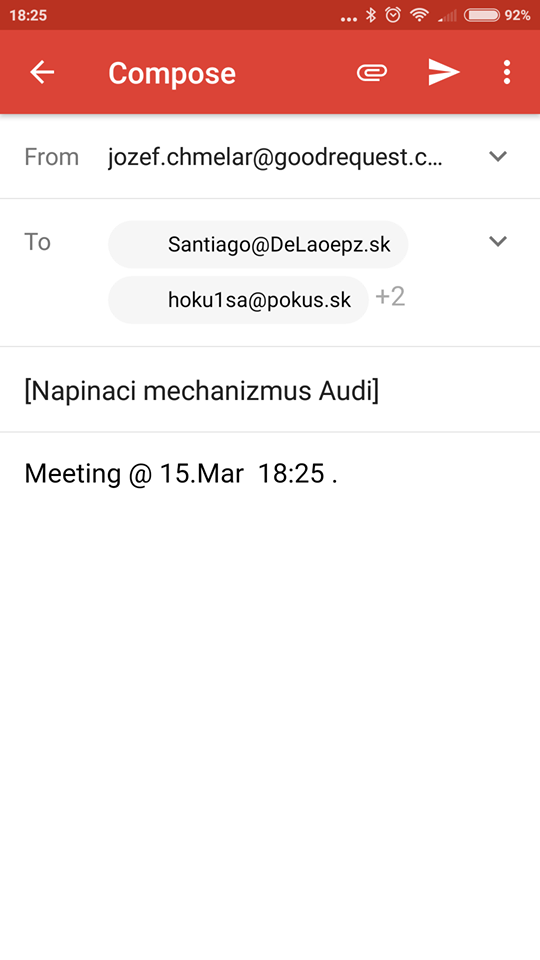
\includegraphics[width=0.4\textwidth]{images/screenz/meeting_mail.png}\label{obr3.10}}
    \caption{Obrazovky stretnutia}

\end{figure}

\subsection{Služobné cesty}
Obrazovka ktorá poskytuje prehľad všetkých pracovných ciest, s dôvodom cesty, autom a dátumom. Po kliknutí na špecifickú cestu sa zobrazí detail so zúčastnenými osobami. Po kliknutí na tlačítko s logom auta sme presmerovaný na obrazovku ktorá umožňuje pridanie novej cesty. Tu využijeme polia s automatickým dopĺňaním textu, a dialógu na výber dátumu
\vspace{10pt}
\begin{figure}[H]
  \centering
  \subfloat[Prehľad služobných ciest]{
    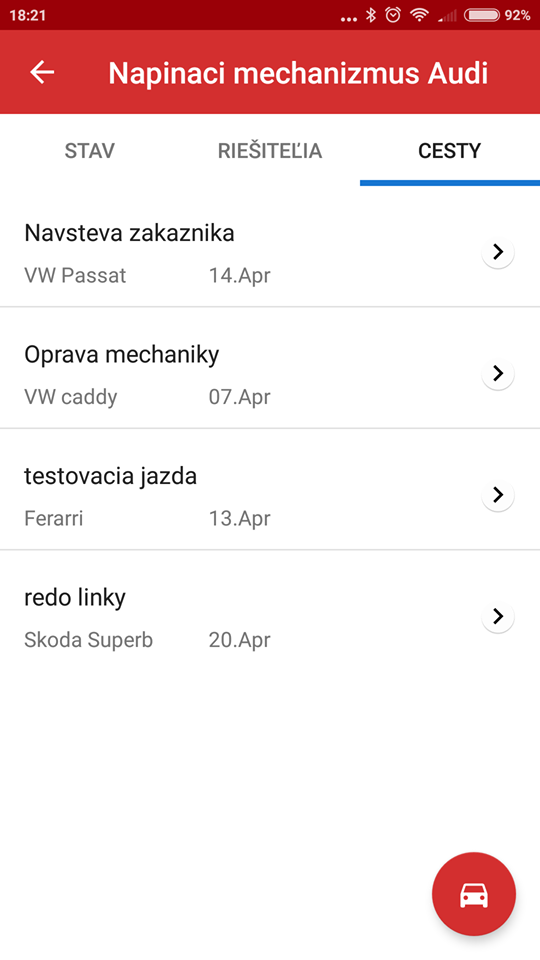
\includegraphics[width=0.4\textwidth]{images/screenz/cesty.png}\label{obr3.11}
  }
  \hfill
  \subfloat[Pred-vyplnený email]{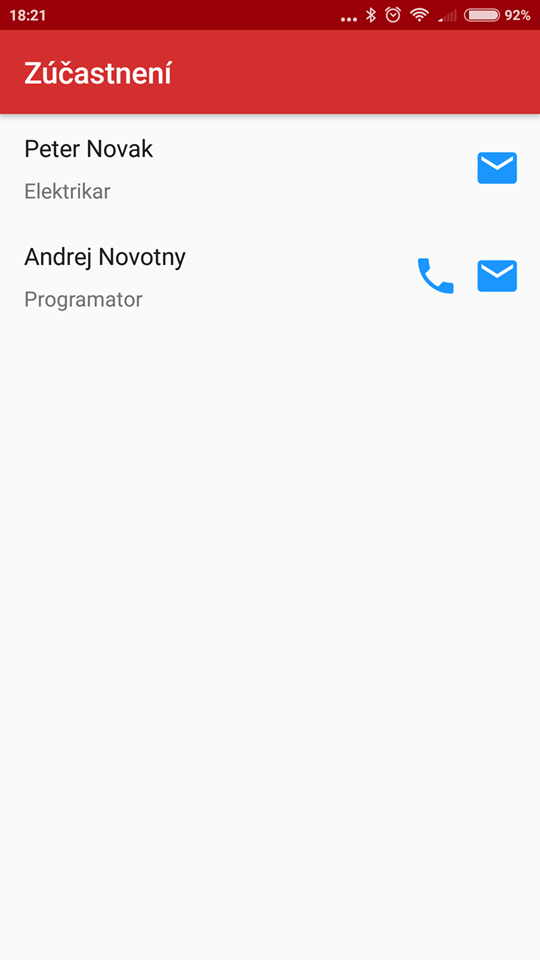
\includegraphics[width=0.4\textwidth]{images/screenz/cesty_zucastneni.png}\label{obr3.10}}
    \caption{Detail služobnej cesty}
\end{figure}

\vspace{10pt}

\section{Serverová časť}

Aplikácia musí fungovať z akejkoľvek siete bez nutnosti využívať VPN (virtual private network) na prístup do firemnej siete, rozhodli sme sa teda pre využitie zadarmo prístupných služieb \textit{Heroku}  ktoré poskytuje hosting pre NodeJS aplikáciu, ktorá je naprogramovaná použitím frameworku ExpressJS, ktorý uľahčuje prácu pri vytvárani REST API. Aplikácia je napojená na databázu ktorú poskytuje server \textit{Mlab.com}. Jedná sa o bezplatnú inštanciu  noSQL databázy MongoDB. MongoDB je vhodný nástroj, pretože na komunikáciu medzi zariadeniami používame formát JSON, ktorý je prirodzený pre Mongo,Node.JS a najpoužívanejší pre REST API. API poskytuje koncové body na vytváranie, editovanie, mazanie a získavanie dát z databázy.

\subsection{Bezpečnosť}

Dôležitou súčasťou každej aplikácie je bezpečnosť a zamedzenie prístupu neoprávneným osobám k citlivým dátam. Framework s ktorým pracujem, \textit{Express.JS}, poskytuje funkciu zvanú ``middleware''\cite{express}, ktorá umožňuje narušiť cyklus požiadavky. Pri každej požiadavke na server sa spustí práve táto funkcia, ktorá hľadá v hlavičke požiadavky kľúč \textit{x-access-token}. Ak je dekódovaný kľuč platný, funkcia zavolá metódu \textit{next()}, ktorá spustí požadovaný proces. Pokiaľ kľúč nie je platný, server odpovie Http kódom 403, prístup zamietnutý. 

Pri vytvorení nového používateľa sa do databázy ukladá zakódovaná verzia jeho hesla. Hash hesla je generovaný pomocou knižnice JWT a bcrypt. Každé heslo je ``osolené'' náhodným a tajným reťazcom znakov, ktorý je uložený ako premenná prostredia na Heroku. Pokiaľ majú dvaja užívatelia rovnaké heslo, nie sme to schopní zisiť pri pohľade na tabuľku užívateľov v databáze, keďže sú uložené ako úplne odlišné 60 znakové reťazce.

\subsection{Databáza}

Ako databázový systém bol zvolená  noSQL databáza MongoDB, ktorej inštanciu nám poskytuje služba mLab. Aplikácia sa po spustení na serveri okamžite pripája k databázovej URL, ktorá je  uložená na Heroku v premenných prostredia, pretože obsahuje meno a heslo potrebné k pripojeniu. Následne komunikujeme s databázou pomocou \textit{ORM Mongoose}. \textit{ORM} automaticky mení odpoveď databázy na objekt, vyhľadáva, filtruje a automaticky spája tabuľky pomocou cudzieho kľúča. MongoDB nie je relačná databáza, označuje sa termínom noSQL  - ``not only SQL''. Nie je viazaná modelom a môže byť kedykoľvek zmenená, nezaručuje teda konzistentnosť dát. Preto používame objekty typu \textit{commentSchema}. V schéme  definujeme štruktúru dát a referencie na ostatné tabuľky.
\vspace{10pt}

\begin{lstlisting}[language=JavaScript]
var commentSchema = new Schema({	
    author: {type: Number , ref:'Employee', required: true},
    text: { type: String, required: true },    
    createdAt: {type: Date,  default: Date.now}
}
\end{lstlisting}

Ako príklad, použijeme najjednoduchšiu schému \textit{commentSchema}. Obsahuje referenciu na tabuľku \textit{Employee} s rovnakým typom ako je primárny kľúč v odkazovanej tabuľke. Automaticky je vytvorená aj premenná \textit{objectId}, ktorá je jednoznačným identifikátorom  pre \textit{commentSchema}. 
\vspace{10pt}


\begin{figure}[H]
    \begin{center}
        \begin{minipage}{0.7\linewidth}
            \begin{center}
     \frame{            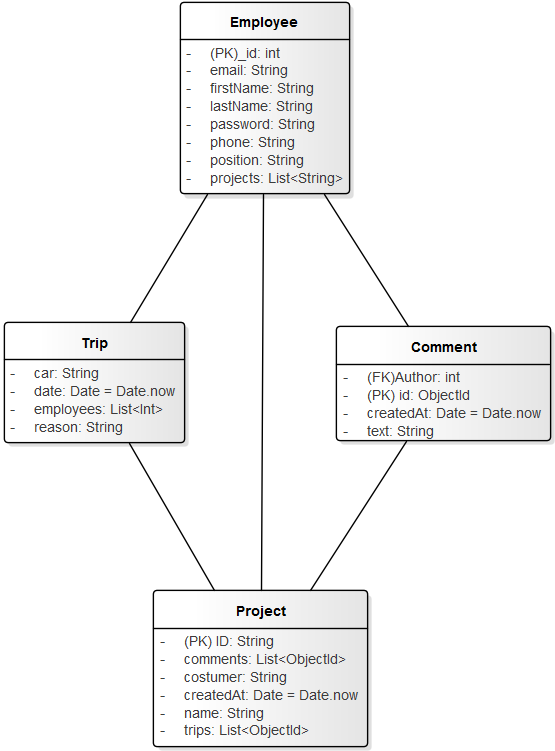
\includegraphics[width=1\textwidth]{images/dbModel.png} }
                \caption{Model databázy}
                \label{obr4.12}
            \end{center}
        \end{minipage}
    \end{center}
\end{figure}


